\section{Introduction}

\subsection{Contexte}
Dans le cadre de la formation de microtechnicien, l'étudiant doit réaliser un Travail de Bachelor pour valider ses compétences. Ainsi, ce travail se déroule en collaboration avec le laboratoire Swiss Cat + de l'EPFL. Le projet doit être réalisé sur une durée de 420 heures, réparties entre mi février et la fin du mois de juillet.

\vspace{0.3cm}
Le laboratoire Swiss Cat + est "une infrastructure axée sur les données
pour la découverte et l'optimisation des catalyseurs" d'après le site internet \cite{swisscatweb}.

L'objectif principal du laboratoire est l'automatisation robotique à haut débit d'expérimentation dans le domaine de la chimie, combinée à une analyse avancée soutenue par l'intelligence artificielle.

\vspace{0.3cm}
Le projet est subdivisé en deux hubs l'un se concentre sur la catalyse homogène à EPFL et l'autre sur la catalyse hétérogène à l'ETHZ.

\begin{figure}[H]
    \centering
    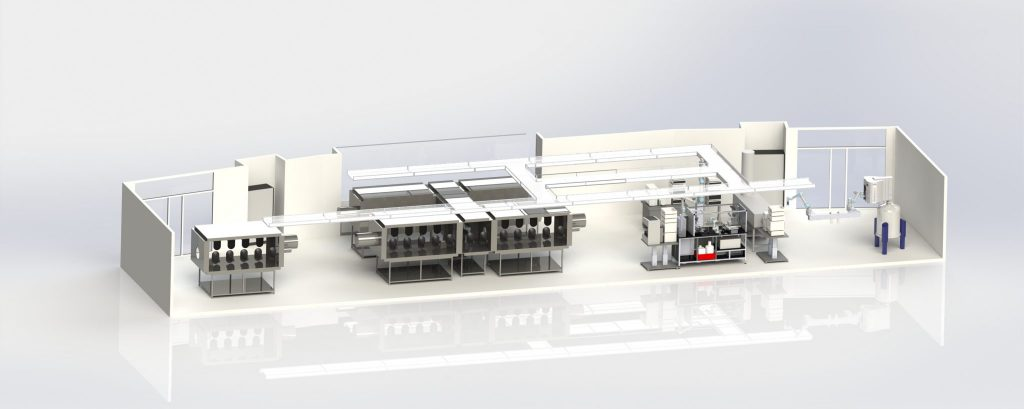
\includegraphics[width=13cm]{Images/Illustrations/Intro/Labo_swisscat_vue3D.jpg}
    \label{fig:Labo-Vue-3D}
    \caption{Vue d'ensemble du laboratoire Swiss Cat + sur le campus EPFL}
\end{figure}

\subsection{Description du projet}
Le projet du TB, intervient au sein du projet StoRMS, une solution innovant visant à préparer des solutions chimiques de manière automatisé, par la manipulation de micro-capsules de réactifs chimiques solides. 

\vspace{0.3cm}
Les micro-capsules permettent de stocker les différentes quantités de réactif de manière imprécise. Dans un second temps, on mesure leurs masses, puis on combine plusieurs micro-capsules pour obtenir la quantité exacte de réactif nécessaire pour la réaction chimique.

\vspace{0.3cm}
Cependant, ces micro-capsules sont celées lors de leur remplissage, il est donc nécessaire de les ouvrir pour libérer le réactif. C'est à ce moment que le système de destruction de micro-capsules entre en jeu.

\subsection{Organisation}
Le document est divisé comme suit:
\begin{itemize}[label=\textbullet]
    \item \textbf{Introduction}: Présentation du projet et de son contexte.
    \item \textbf{Analyse du besoin}: Identification des besoins du système.
    \item \textbf{Fonctions et exigences du système}: Définition des fonctions de services et techniques du système.
    \item \textbf{Catalogue des solutions}: Présentation des solutions techniques envisagées.
    \item \textbf{Modélisation 3D et réalisation}: Description de la réalisation du système.
    \item \textbf{Tests et validation}: Présentation des tests effectués et des résultats obtenus.
    \item \textbf{Conclusion}: Bilan du projet et perspectives d'amélioration.
\end{itemize}
\newpage